\section{Docker Security}
\label{sec::security}

% 4. Docker security
%     1. UID 0
%     2. Privileged Containers
%     3. Secure Computing Mode
%     4. SElinux and AppArmor

\subsection{cgroups}
\label{ssec::security:cgroups}

Docker relies on cgroups to limit a container's resources, such as memory, swap, \acs{CPU}, storage and network I/O. cgroups are built into the Linux kernel and this mechanism assures that one container process can't affect the performance of the other processes running on the host machine. In the official kernel documentation it is defined as:
\begin{displayquote}
    \textit{"A mechanism for aggregating/partitioning sets of tasks and all their future children into hierarchical groups with specialized behavior."}
\end{displayquote}
This hierarchy can be displayed in the figure \ref{fig:cgroup-hch}.

\begin{figure}[!htb]
    \centering
    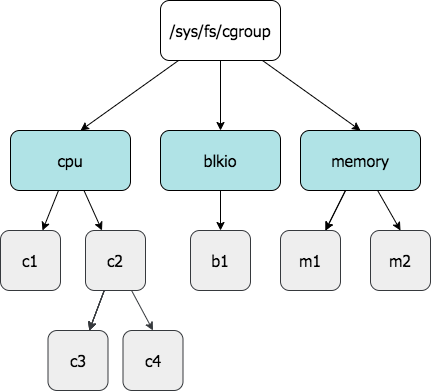
\includegraphics[width=0.25\textwidth]{cgroup.png}
    \caption{Scheme representing Linux cgroup hierarchy\cite{fig-src:cgroups}. Here, the \acs{CPU} resources are split across two tasks, the latter having two child processes. The process \texttt{c3}, for instance, cannot access resources allocated for neither \texttt{c4} or \texttt{c1}. It is constrained to the resources inherited from \texttt{c2}.}
    \label{fig:cgroup-hch}
\end{figure}

When a container is created, Docker automatically assigns a cgroup unique to that container and all the processes of that container will be in the same group.

Constraining resources protects against a class of attacks that attempt to disrupt the system by consuming excessive resources, starving the legitimate applications. It's recommended to set CPU and memory limits in each container when deploying container applications.


\subsection{Namespaces}
\label{ssec::security:namespaces}

\placeholder{Begin draft}

Kernel namespaces are at the very heart of containers! They let us slice up an operating system (OS) so that it looks and feels like multiple isolated operating systems.

namespaces control what it can see. By putting a process in a namespace, you can restrict the resources that are visible to that process.

Unix systems allowed the mounting of filesystems, but they would all be mounted into the same system-wide view of all filenames. In Plan 9, each process was part of a process group that had its own “name space” abstraction, the hierarchy of files (and file-like objects) that this group of processes could see. Each process group could mount its own set of file systems without seeing each other.

There are several different kinds of namespace supported by Linux:
\begin{itemize}
    \item Unix Timesharing System (UTS)—this sounds complicated, but to all intents and purposes this namespace is really just about the hostname and domain names for the system that a process is aware of.
    \item Process IDs
    \item Mount points
    \item Network
    \item User and group IDs
    \item Inter-process communications (IPC)
    \item  Control groups (cgroups)
\end{itemize}

Let's briefly look at how Docker uses each namespace:
\begin{itemize}
    \item Process ID namespace: Docker uses the pid namespace to provide isolated process trees for each container. Every container gets its own process tree, meaning that every container can have its own PID 1. PID namespaces also mean that a container cannot see or access to the process tree of other containers, or the host it's running on.
    \item Network namespace: Docker uses the net namespace to provide each container its own isolated network stack. This stack includes; interfaces, IP addresses, port ranges, and routing tables. For example, every container gets its own eth0 interface with its own unique IP and range of ports.
    \item Mount namespace: Every container gets its own unique isolated root / filesystem. This means that every container can have its own /etc, /var, /dev etc. Processes inside of a container cannot access the mount namespace of the Linux host or other containers — they can only see and access their own isolated mount namespace.
    \item Inter-process Communication namespace: Docker uses the ipc namespace for shared memory access within a container. It also isolates the container from shared memory outside of the container.
    \item User namespace: Docker lets you use user namespaces to map users inside of a container to different users on the Linux host. A common example is mapping the root user of a container to a non-root user on the Linux host.
    \item User namespaces are quite new to Docker and currently optional. This may change in the future.
    \item UTS namespace: Docker uses the uts namespace to provide each container with its own hostname.  By putting a process in its own UTS namespace, you can change the hostname for this process independently of the hostname of the machine or virtual machine on which it's running The container can have its own hostname because Docker created it with its own UTS namespace
\end{itemize}

\subsection{UID 0}
\label{ssec::security:uid0}

The user namespace allows processes to have their own view of user and group IDs. Much like process IDs, the users and groups still exist on the host, but they can have different IDs. The main benefit of this is that you can map the root ID of 0 within a container to some other non-root identity on the host. This is a huge advantage from a security perspective, since it allows software to run as root inside a container, but an attacker who escapes from the container to the host will have a non-root, unprivileged identity.

User namespaces allow an unprivileged user to effectively become root within the
containerized process. This allows a normal user to run containers using a concept called rootless containers, The general consensus is that user namespaces are a security benefit because fewer containers need to run as “real” root

\subsection{Privileged Containers}
\label{ssec::security:priv-cont}

\placeholder{TODO}

\subsection{Secure Computing Mode}
\label{ssec::security:sec-compt}
\placeholder{TODO}

\subsection{Mandatory Access Control}
\label{ssec::security:sel-apparm}

Using mandatory access controls gives the administrator much more granular control of what can happen on their system, in a way that individual users can't override.

\subsubsection{\textbf{AppArmor}}
AppArmor (short for “Application Armor”) is one of a handful of Linux security
modules (LSM) that can be enabled in the Linux kernel. In AppArmor, a profile can be associated with an executable file, determining what that file is allowed to do in terms of capabilities and file access permissions. AppArmor and other LSMs implement mandatory access controls. A mandatory access control is set by a central administrator, and once set, other users do not have any ability to modify the control or pass it on to another user.

AppArmor includes a “complain” mode in which you can run your executable against a profile and any violations get logged. The idea is that you can use these logs to update the profile, with the goal of eventually seeing no new violations, at which point you start to enforce the profile.

\subsubsection{\textbf{SELinux}}
SElinux lets you constrain what a process is allowed to do in terms of its interactions with files and other processes. Each process runs under an SELinux domain—you can think of this as the context that the process is running in—and every file has a type.

A key distinction between SELinux permissions and regular DAC Linux permissions is that in SELinux, permissions have nothing to do with the user identity—they are described entirely by labels. That said, they work together, so an action has to be permitted by both DAC and SELinux.

Creating an effective SELinux profile for an application takes in-depth knowledge of the set of files that it might need access to, in both happy and error paths, so that task may be best left to the app developer. Some vendors provide profiles for their applications.



\placeholder{End draft}